\documentclass[a4paper,12pt]{article}
\usepackage[utf8]{inputenc} %codification of the document
\usepackage{mathtools}
\usepackage{amsfonts}
\usepackage{amsmath}
\usepackage{tikz}
\usepackage{tikz-3dplot} 

\begin{document}

\title{Vector}
% \maketitle

\section*{Introduction to Vector}
\begin{itemize}
  \item Definition
  \item[] Vector is the quantity that has a \textbf{magnitude} and a \textbf{direction}.
  \item Notation
  \item[] $\overrightarrow{AB} = \overrightarrow{a} = \textbf{a} $
  \item[] $\textbf{v} = (v_1, v_2) = \begin{pmatrix} v_1 \\ v_2 \end{pmatrix} $
  \item[] 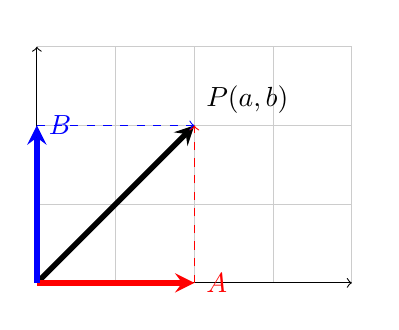
\begin{tikzpicture}
      \draw[thin,gray!40] (0,0) grid (4,3);
      \draw[->] (0,0)--(4,0) node[right]{};
      \draw[->] (0,0)--(0,3) node[above]{};
      \draw[line width=2pt,black,-stealth](0,0)--(2,2) node[anchor=south west]{$P(a,b)$};
      \draw[line width=2pt,red,-stealth](0,0)--(2,0) node[anchor=west]{$A$};
      \draw[line width=2pt,blue,-stealth](0,0)--(0,2) node[anchor=west]{$B$};
      \draw[dashed, blue ,->](0,2)--(2,2) node[anchor=west]{};
      \draw[dashed, red,->](2,0)--(2,2) node[anchor=west]{};
    \end{tikzpicture}
\end{itemize}

\section*{Zero Vector and Equal Vector}

\subsection*{Zero Vector}
\begin{itemize}
  \item A zero vector, denoted \textbf{0}, is a vector of length 0, and thus has all components equal to zero.
  \item[] \textbf{0} = (0, 0) (vector in R2)
  \item[] \textbf{0} = (0, 0, 0) (vector in R3)
  \item Zero vector parallel with all vector
\end{itemize}

\subsection*{Unit Vector}
\begin{itemize}
  \item Unit vector is a vector of length 1
  \item[] \(\hat{u}=\frac{\textbf{u}}{|\textbf{u}|}\)
\end{itemize}


\subsection*{Equal Vector}
\begin{itemize}
  \item Equal vectors are vectors that have the \textbf{same magnitude} and the \textbf{same direction}, but the coordinates can be different.
  \item Two vectors are equal if and only if their corresponding components are equal.
  \item[] \(\begin{pmatrix} a_1 \\ a_2 \end{pmatrix} = \begin{pmatrix} b_1 \\ b_2 \end{pmatrix}\), if and only if \(a_1 = b_1\) and \(a_2 = b_2\)
\end{itemize}

\section*{Vector Arithmetic}
\subsection*{Addition and Subtraction}
\begin{itemize}
  \item If \textbf{v} and \textbf{w} are any two vectors, then the sum \(\textbf{v} + \textbf{w}\) is the vector determined as follows: Position the vector \textbf{w} so that its initial point coincides with the terminal point of \textbf{v}. The vector is represented by the arrow from the initial point of \textbf{v} to the terminal point of \textbf{w}.
  \item If \textbf{v} and \textbf{w} are any two vectors, then the difference of \textbf{w} from \textbf{v} is defined by \(\textbf{v}-\textbf{w}=\textbf{v}+(-\textbf{w})\)
  \item If \(\textbf{v}=(v_1, v_2)\) and \(\textbf{w}=(w_1, w_2)\), then \(\textbf{v}\pm\textbf{w}=(v_1\pm w_1, v_2\pm w_2)\)
  \item In set of vectors S in the plane, the sum is closed if: \begin{itemize}
          \item The result of the sum of two defined (any) and single vectors
          \item The result of the sum is included in the set H.
        \end{itemize}
\end{itemize}
\subsection*{Scalar Multiplication}
\begin{itemize}
  \item If \textbf{v} is a nonzero vector and \(k\) is a scalar number, then the product \(k\textbf{v}\) is defined to be the vector whose length is \(|k|\) times the length of \textbf{v} and whose direction is the same as that of \textbf{v} if \(k>0\) and opposite to that of \textbf{v} if \(k<0\). We define \(k\textbf{v}=0\) if \(k=0\) or \(\textbf{v}=0\).
  \item If \(\textbf{v}=(v_1, v_2)\) and \(k\) is any scalar, then \(k\textbf{v}=(kv_1, kv_2)\)
  \item If a vector \textbf{v} is the product of a vector \textbf{w} by a scalar, then the vectors \textbf{v} and \textbf{w} are parallel.
\end{itemize}

\subsection*{Properties of Vector Arithmetic}
With the explanation above, if \textbf{u}, \textbf{v}, and \textbf{w} are vectors in 2- or 3-space and \(k\) and \(l\) are scalars, then the following relationships hold.
\begin{itemize}
  \item \(\textbf{u}+\textbf{v}=\textbf{v}+\textbf{u}\)
  \item \((\textbf{u}+\textbf{v})+\textbf{w}=\textbf{u}+(\textbf{v}+\textbf{w})\)
  \item \(\textbf{u}+0=0+\textbf{u}\)
  \item \(\textbf{u}+(-\textbf{u})=0\)
  \item \(k(l\textbf{u})=kl(\textbf{u})\)
  \item \(k(\textbf{u}+\textbf{v})=k\textbf{u}+k\textbf{v}\)
  \item \((k+l)\textbf{u}=k\textbf{u}+k\textbf{v}\)
  \item \(l\textbf{u}=\textbf{u}\)
\end{itemize}

\subsection*{Norm of A Vector}
The length of a vector \textbf{u} is often called the norm of \textbf{u} and is denoted by \(||\textbf{u}||\).
\begin{itemize}
  \item For vector in 2-space, \(||\textbf{v}||=\sqrt{{v_1}^2+{v_2}^2}\)
  \item For vector in 3-space, \(||\textbf{v}||=\sqrt{{v_1}^2+{v_2}^2+{v_3}^2}\)
\end{itemize}
With this, one can find distance \(d\) between two vectors as :
\begin{itemize}
  \item For vector in 2-space, \(d=\sqrt{(v_1-w_1)^2+(v_2-w_2)^2}\)
  \item For vector in 3-space, \(d=\sqrt{(v_1-w_1)^2+(v_2-w_2)^2+(v_3-w_3)^2}\)
\end{itemize}

\subsection*{Dot Product}
\subsubsection*{Definition}
\begin{enumerate}
  \item If \(\alpha\) is angle between \textbf{a} and \textbf{b}, then: \begin{center}
          \(\textbf{a}.\textbf{b}=\begin{cases}
            \text{0 if $\textbf{a} = 0$ or $\textbf{b} = 0$} \\
            \text{$||\textbf{a}||||\textbf{b}||\cos\alpha$, with $0\ge\alpha\ge\pi$}
          \end{cases} \)
        \end{center}
  \item If \textbf{a} and \textbf{b} are vector in \(R^2\), then \(\textbf{a}.\textbf{b}=a_1b_1+a_2b_2\)
  \item[] Similar to above, in \(R^3\), \(\textbf{a}.\textbf{b}=a_1b_1+a_2b_2+a_3b_3\)
\end{enumerate}
Note that if \textbf{a}, \textbf{b}, and \textbf{c} are vectors, then \((\textbf{a}.\textbf{b}).\textbf{c}\neq\textbf{a}.(\textbf{b}.\textbf{c})\) because dot product output a scalar number, and scalar numbers cannot be dot product with vector

\subsubsection*{Properties}
\begin{itemize}
  \item \(\textbf{u}.\textbf{v}=\textbf{v}.\textbf{u}\)
  \item \((k\textbf{u}).\textbf{v}=k(\textbf{u}.\textbf{v})\)
  \item \(\textbf{u}(\textbf{v}+\textbf{w})=\textbf{u}.\textbf{v}+\textbf{u}.\textbf{w}\)
  \item \(\textbf{v}.\textbf{v}=\begin{cases}
          ||\textbf{v}||||\textbf{v}|| \\
          0 & \text{if $\textbf{v}=0$}
        \end{cases}\)
\end{itemize}

\subsubsection*{Angle and Result of Dot Product}
\begin{itemize}
  \item Pay attention to the equation \(||\textbf{a}||||\textbf{b}||\cos\alpha\).
  \item Norm of a vector will always be greater than or equal to 0, but \(\cos\alpha\) can be positive, negative or 0 depending on the value of \(\alpha\).
  \item[] \(\textbf{u}.\textbf{v}=\begin{cases}
      \text{$<0$} & \text{if $\alpha > \frac{\pi}{2}$}                 \\
      \text{$=0$} & \text{if \textbf{u} and \textbf{v} are orthogonal} \\
      \text{$>0$} & \text{if $\alpha < \frac{\pi}{2}$}                 \\
    \end{cases}\)
\end{itemize}

\subsubsection*{Dot Product and Matrix Multiplication}
\begin{itemize}
  \item Pay attention to the equation \(\textbf{a}.\textbf{b}=a_1b_1+a_2b_2\)
  \item If \textbf{a} and \textbf{b} seen as matrices \(A\) and \(B\) respectively, then:
  \item[] \(\textbf{a}.\textbf{b}=a_1b_1+a_2b_2=\begin{bmatrix}a_1, a_2\end{bmatrix}\begin{bmatrix}b_1 \\ b_2\end{bmatrix}=A.B^T\)
\end{itemize}

\subsection*{Orthogonal Projection}
\subsubsection*{Orthogonal Projection on The Axis}
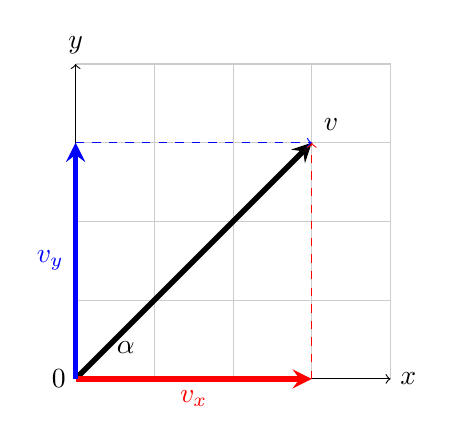
\begin{tikzpicture}
  \draw[thin,gray!40] (0,0) grid (4,4);
  \draw[->] (0,0)--(4,0) node[right]{$x$};
  \draw[->] (0,0)--(0,4) node[above]{$y$};
  \draw[] (0,0) node[left]{$0$};
  \draw[] (0.4,0.4) node[right]{$\alpha$};
  \draw[line width=2pt,black,-stealth](0,0)--(3,3) node[anchor=south west]{$v$};
  \draw[line width=2pt,red,-stealth](0,0)--(3,0) node[midway,below]{$v_x$};
  \draw[line width=2pt,blue,-stealth](0,0)--(0,3) node[midway,left]{$v_y$};
  \draw[dashed, blue ,->](0,3)--(3,3) node[anchor=west]{};
  \draw[dashed, red,->](3,0)--(3,3) node[anchor=west]{};
\end{tikzpicture}
\begin{itemize}
  \item \(v_x\) is the orthogonal projection of \textbf{v} on the \(x\)-axis
  \item \(v_y\) is the orthogonal projection of \textbf{v} on the \(y\)-axis
  \item So by definition: \begin{itemize}
          \item \(\textbf{v} = v_x + v_y\)
          \item \(|v_x|=|\textbf{v}|\cos\alpha\)
          \item \(|v_y|=|\textbf{v}|\sin\alpha\)
        \end{itemize}
  \item \textbf{v} can be decomposed into the sum of two vectors, \(v_x\) and \(v_y\)
\end{itemize}

\subsection*{Orthogonal Projection and Decomposition}
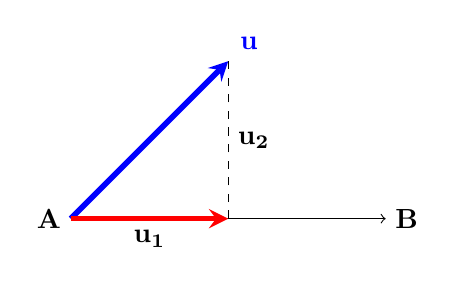
\begin{tikzpicture}
  \draw[] (0,0) node[left]{\textbf{A}};
  \draw[->] (0,0)--(4,0) node[right]{\textbf{B}};
  \draw[line width=2pt,blue,-stealth](0,0)--(2,2) node[anchor=south west]{\textbf{u}};
  \draw[line width=2pt,red,-stealth](0,0)--(2,0) node[midway,black,below]{\textbf{u\(_\textbf{1}\)}};
  \draw[dashed, black,-](2,0)--(2,2) node[midway,anchor=west]{\textbf{u\(_\textbf{2}\)}};
\end{tikzpicture}
\begin{itemize}
  \item The vector \textbf{u\(_\textbf{1}\)} is called the \textbf{orthogonal projection of u} on \(A\) or sometimes the vector component of \textbf{a} along \(A\). It is denoted by \begin{center}
          \(\text{proj}_\textbf{a}\textbf{u} = \frac{\textbf{u}.\textbf{b}}{||\textbf{b}||^2}.\textbf{b}\)
        \end{center}
  \item The vector \textbf{u\(_\textbf{2}\)} is called the \textbf{vector component of u orthogonal to a}. Since \(\textbf{u}_\textbf{2}=\textbf{u}-\textbf{u}_\textbf{1}\), this vector can be written as \begin{center}
          \(\textbf{u}-\text{proj}_\textbf{a}\textbf{u} = \textbf{u}-\frac{\textbf{u}.\textbf{b}}{||\textbf{b}||^2}.\textbf{b}\)
        \end{center}
\end{itemize}

\subsection*{Cross Product}
\begin{itemize}
  \item Given two vectors \textbf{a} and \textbf{b}, the cross product of \textbf{a} and \textbf{b}, denoted by \(\textbf{a}\times\textbf{b}\), is another vector that is perpendicular to both \textbf{a} and \textbf{b}.
  \item Suppose there are two vectors, \(\textbf{u}=(u_1,u_2,u_3)\) and \(\textbf{v}=(v_1,v_2,v_3)\), then \begin{center}
          \(\textbf{u}\times\textbf{v}=((u_2v_3-u_3v_2), (u_3v_1-u_1v_3), (u_1v_2-u_2v_1))\)
        \end{center}
        or in determinant notation, \begin{center}
          \(\textbf{u}\times\textbf{v}=\Big(\text{det}\begin{vmatrix}
            u_2 & u_3 \\ v_2 & v_3
          \end{vmatrix}, -\text{det}\begin{vmatrix}
            u_1 & u_3 \\ v_1 & v_3
          \end{vmatrix}, \text{det}\begin{vmatrix}
            u_1 & u_2 \\ v_1 & v_2
          \end{vmatrix}\Big)\)
        \end{center}
\end{itemize}

\subsubsection*{Properties}
\begin{itemize}
  \item \(\textbf{u}\times\textbf{v}=-\textbf{v}\times\textbf{u}\)
  \item If \textbf{u} parallel with \textbf{v}, then \(\textbf{u}\times\textbf{v}=-\textbf{v}\times\textbf{u}=0\)
  \item \((k\textbf{u})\times\textbf{v}=\textbf{u}\times(k\textbf{v})=k(\textbf{u}\times\textbf{v})\)
  \item \(\textbf{u}\times(\textbf{v}+\textbf{w})=\textbf{u}\times\textbf{v}+\textbf{u}\times\textbf{w}\)
  \item \(\textbf{u}.(\textbf{v}\times\textbf{w})=(\textbf{u}\times\textbf{v}).\textbf{w}\)
\end{itemize}

\end{document}